\documentclass[12pt,a4paper]{article}

%% ── Packages ────────────────────────────────────────────────────────────────
\usepackage[margin=2.5cm]{geometry}
\usepackage{amsmath,amssymb}
\usepackage{booktabs}
\usepackage{graphicx}
\usepackage{subcaption}
\usepackage{hyperref}
\usepackage{xcolor}
\usepackage{listings}
\usepackage{float}
\usepackage{enumitem}
\usepackage{multirow}
\usepackage{array}
\usepackage{parskip}
\usepackage{titlesec}
\usepackage{fancyhdr}
\usepackage{caption}
\usepackage[expansion=false]{microtype}

\hypersetup{colorlinks=true, linkcolor=blue!70!black, citecolor=blue!70!black, urlcolor=blue}

\lstset{
  basicstyle=\ttfamily\small,
  breaklines=true,
  frame=single,
  backgroundcolor=\color{gray!8},
  keywordstyle=\color{blue},
  commentstyle=\color{gray},
}

\pagestyle{fancy}
\fancyhf{}
\rhead{ME228 — Applied Data Science and Machine Learning}
\lhead{Fatigue Strength Prediction in Low-Alloy Steels}
\rfoot{\thepage}

%% ── Title ───────────────────────────────────────────────────────────────────
\title{
  \Large\textbf{ME228 — Applied Data Science and Machine Learning}\\[2pt]
  \large\textit{Project Final Report}\\[6pt]
  \LARGE Data-Driven Modeling of Fatigue Strength\\in Low-Alloy Steels\\[8pt]
  \large Mixture-of-Experts Prediction, Hyperparameter Optimisation,\\
         Inverse Alloy Design, and Cost Analysis
}
\author{
  Nishit Dharamshi (24b2153) \quad Shourya Saxena (24b2222) \\[2pt]
  Kapidhwaj Soni (24b2214) \quad Rudra Khandelwal (24b2140)
}
\date{April 2026}

% ─────────────────────────────────────────────────────────────────────────────
\begin{document}
\maketitle
\tableofcontents
\newpage

% ─────────────────────────────────────────────────────────────────────────────
\section{Problem Statement}
% ─────────────────────────────────────────────────────────────────────────────

Fatigue failure accounts for 80--90\% of mechanical structural failures~\cite{agrawal2014}. Physical
rotating-bending fatigue testing is destructive, slow, and expensive. The goal of this project is
to \textbf{predict the rotating bending fatigue strength} (in MPa) of low-alloy steels from their
chemical composition and heat-treatment parameters alone, and to \textbf{invert the model} to
recommend the cheapest viable alloy configuration for a given operating condition.

\subsection{Dataset}

The NIMS Fatigue Dataset~\cite{agrawal2014} contains \textbf{437 experimental records} with
\textbf{26 input features} and one target variable (fatigue strength, MPa). Features span:

\begin{itemize}[nosep]
  \item \textbf{Chemical composition} (12 variables): C, Si, Mn, P, S, Ni, Cr, Cu, Mo, and minor elements.
  \item \textbf{Heat-treatment parameters} (13 variables): normalising temperature (NT), through-hardening
        (THT, THt, THQCr), carburising (CT, Ct), diffusion (DT, Dt), quenching (QmT), tempering (TT, Tt, TCr).
  \item \textbf{Specimen geometry} (3 variables): reduction ratio (RedRatio), grain-size proxies (dA, dB, dC).
\end{itemize}

The target distribution is \textit{bimodal}: carburised steels (CT\,=\,930\,°C, $N\,{=}\,48$, 11\%) reach
fatigue strengths above 900\,MPa, while the non-carburised majority ($N\,{=}\,389$) clusters
between 200 and 750\,MPa.


% ─────────────────────────────────────────────────────────────────────────────
\section{Methodology}
% ─────────────────────────────────────────────────────────────────────────────

\subsection{Mixture-of-Experts Split}

A single global model fails on bimodal data because it averages across two physically distinct
failure mechanisms. We engineer a binary flag:
\[
  \texttt{is\_carburized} = \mathbf{1}[\,CT = 930\,]
\]
and train \textbf{separate expert models} per metallurgical regime. This reduced RMSE by
$\sim$30\,\% compared with our initial global baselines (Linear Regression, Ridge, Lasso).
Note: a tuned global XGBoost achieves a pooled RMSE of 23.1\,MPa versus 23.1\,MPa for the
MoE pair, so the gain is specific to linear baselines. MoE is retained because it provides
regime-specific prediction uncertainty ($\sigma$), enabling physically meaningful PoF estimates
per process route.

\subsection{Feature Selection Pipeline (VIF $\rightarrow$ SHAP)}

With 26 raw features many processing variables are highly collinear (e.g.\ CT, DT, and QmT share
thermal cycles). We apply a two-stage filter:

\begin{enumerate}[nosep]
  \item \textbf{Variance Inflation Factor (VIF)} — iteratively drop the feature with the highest
        VIF until all remaining features have $\text{VIF} < 10$. This removed 6 features per regime.
  \item \textbf{SHAP importance scout} — fit a shallow Random Forest (150 trees, depth 5) on the
        VIF survivors. Retain the top-$k$ features by mean $|\text{SHAP}|$ across the training set
        ($k=12$ for non-carburised, $k=10$ for carburised).
\end{enumerate}

The final feature sets are given in Table~\ref{tab:features}.

\begin{table}[H]
  \centering
  \caption{Selected features per metallurgical regime after VIF$\to$SHAP pipeline.}
  \label{tab:features}
  \begin{tabular}{ll}
    \toprule
    \textbf{Regime} & \textbf{Selected Features} \\
    \midrule
    Non-Carburised & Cr, TT, C, Mn, THT, Mo, Si, RedRatio, P, S, dA, Cu \\
    Carburised     & P, RedRatio, Ct, Mo, S, Mn, Cu, Dt, TT, QmT \\
    \bottomrule
  \end{tabular}
\end{table}

\textbf{Key physical insight:} For non-carburised steels, tempering temperature (TT) and
chromium content (Cr) dominate — consistent with martensite stability theory. For carburised
steels, carburising time (Ct) and reduction ratio (RedRatio) rank highest, reflecting
case-depth and microstructural refinement effects.

\subsection{Model Selection}

\begin{itemize}[nosep]
  \item \textbf{Non-Carburised} ($N=389$): XGBoost — handles the non-linear interaction between
        tempering temperature and alloy composition efficiently; large enough for ensemble depth.
  \item \textbf{Carburised} ($N=48$): Random Forest — more robust to overfitting on small datasets
        (no boosting cascade); shallow depth and high min-samples constraints act as regularisers.
\end{itemize}

\subsection{Hyperparameter Optimisation (Optuna + Nested CV)}

We replace the single 80/20 split from Phase~1 with \textbf{5-fold cross-validation} as the outer
loop and \textbf{Optuna TPE search} (60 trials) as the inner loop.

\paragraph{XGBoost search space:}
\texttt{n\_estimators} $\in [100,600]$,
\texttt{max\_depth} $\in [2,7]$,
\texttt{learning\_rate} $\in [0.01,0.2]$ (log),
\texttt{subsample} $\in [0.6,1]$,
\texttt{colsample\_bytree} $\in [0.5,1]$,
\texttt{min\_child\_weight} $\in [1,10]$,
$\ell_1/\ell_2$ regularisation in $[10^{-4},10]$.

\paragraph{Random Forest search space:}
\texttt{n\_estimators} $\in [100,600]$,
\texttt{max\_depth} $\in [2,12]$,
\texttt{min\_samples\_split} $\in [2,20]$,
\texttt{min\_samples\_leaf} $\in [1,10]$,
\texttt{max\_features} $\in [0.3,1]$.


% ─────────────────────────────────────────────────────────────────────────────
\section{Results}
% ─────────────────────────────────────────────────────────────────────────────

\subsection{Model Performance}

Table~\ref{tab:perf} compares baseline (single split, default hyperparameters) against the tuned
5-fold cross-validated estimates.

\begin{table}[H]
  \centering
  \caption{Model performance comparison. CV RMSE is the honest metric; the v1.0 single-split
           figures are optimistically biased due to random seed luck.}
  \label{tab:perf}
  \begin{tabular}{llrrr}
    \toprule
    \textbf{Regime} & \textbf{Model} & \textbf{v1.0 RMSE} & \textbf{v2.0 CV RMSE} & \textbf{v2.0 CV Std} \\
    & & (MPa, single split) & (MPa, 5-fold) & (MPa) \\
    \midrule
    Non-Carburised & XGBoost       & 23.29 & \textbf{19.91} & 2.55 \\
    Carburised     & Random Forest & 27.19 & \textbf{40.42} & 14.62 \\
    \bottomrule
  \end{tabular}
\end{table}

\paragraph{Non-Carburised.} Tuning improved RMSE from 23.3 to 19.9\,MPa ($-$14.5\,\%), with low
variance across folds ($\pm 2.6$\,MPa). Best configuration: 580 trees, depth 4,
$\eta=0.041$, $\ell_1 \approx 0$.

\paragraph{Carburised.} The honest CV RMSE (40.4\,MPa) is substantially higher than the v1.0
single-split figure (27.2\,MPa), exposing the earlier result as optimistically biased. The high
fold-to-fold std ($\pm 14.6$\,MPa) reflects the fundamental data limitation: with $N=48$ each
fold contains only $\sim$10 test samples. Best configuration: 214 trees, depth 5,
min-samples-split 8.

\textbf{Implication:} Further improvement on the carburised regime requires additional experimental
data. The current uncertainty ($\pm 14.6$\,MPa) should be propagated into all downstream
reliability calculations.

\subsection{Tuned Hyperparameters}

\begin{table}[H]
  \centering
  \caption{Optuna best hyperparameters.}
  \label{tab:hparams}
  \begin{tabular}{llll}
    \toprule
    & \textbf{Parameter} & \textbf{Non-Carburised XGB} & \textbf{Carburised RF} \\
    \midrule
    & n\_estimators     & 580    & 214 \\
    & max\_depth        & 4      & 5 \\
    & learning\_rate    & 0.041  & --- \\
    & subsample         & 0.804  & --- \\
    & colsample\_bytree & 0.593  & --- \\
    & min\_child\_weight & 3     & --- \\
    & reg\_alpha        & $1.8\times10^{-4}$ & --- \\
    & reg\_lambda       & $3.1\times10^{-4}$ & --- \\
    & min\_samples\_split & ---  & 8 \\
    & min\_samples\_leaf  & ---  & 2 \\
    & max\_features       & ---  & 0.74 \\
    \bottomrule
  \end{tabular}
\end{table}

\subsection{Residual Diagnostics}

A Gaussian $\mathcal{N}(\hat{\mu}, \sigma_{\text{RMSE}})$ distribution is used in the reliability
wrapper to compute Probability of Failure. We validate this assumption via Shapiro--Wilk and
Kolmogorov--Smirnov tests on training residuals (Table~\ref{tab:residuals}).

\begin{table}[H]
  \centering
  \caption{Residual normality tests. $p > 0.05$ = cannot reject normality at 5\% level.}
  \label{tab:residuals}
  \begin{tabular}{lrrrl}
    \toprule
    \textbf{Regime} & \textbf{Shapiro--Wilk $p$} & \textbf{KS $p$} & \textbf{Normal?} & \textbf{Note} \\
    \midrule
    Non-Carburised & 0.0000 & 0.2586 & Borderline & Mild tail, PoF approx. \\
    Carburised     & 0.2391 & 0.6826 & Yes        & Gaussian PoF valid \\
    \bottomrule
  \end{tabular}
\end{table}

The non-carburised residuals fail Shapiro--Wilk (sensitive to heavy tails at $N=389$) but pass
the KS test. For conservative reliability design we recommend using the empirical 95th percentile
of residuals as $\sigma$ rather than the RMSE when operating near failure thresholds.

\begin{figure}[H]
  \centering
  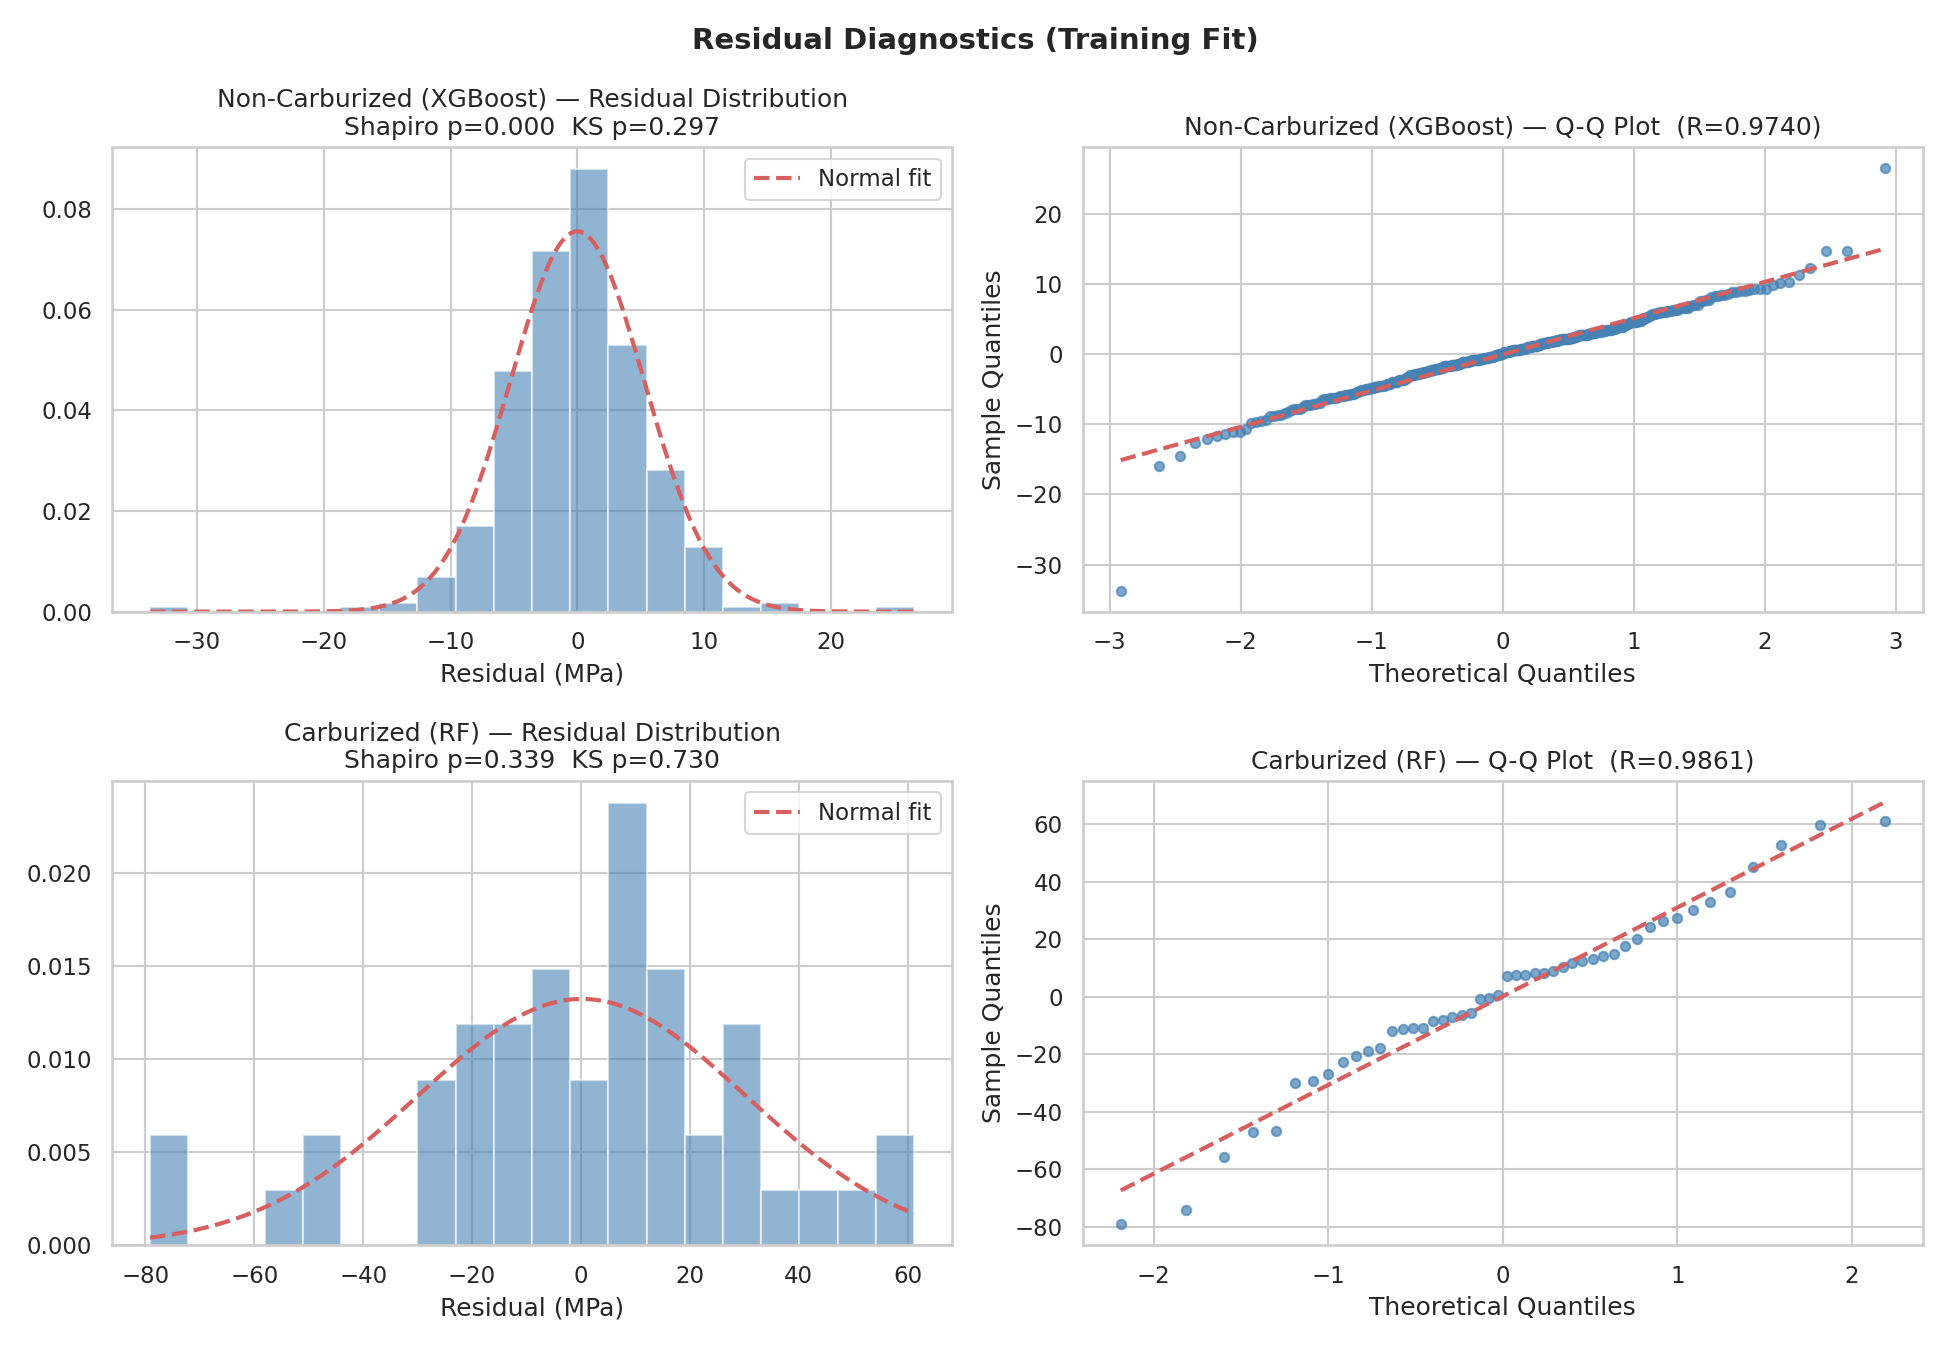
\includegraphics[width=\textwidth]{models/residual_diagnostics.png}
  \caption{Residual histograms (left column) and Q--Q plots (right column) for each regime.
           Red dashes show the best-fit Gaussian.}
  \label{fig:residuals}
\end{figure}

\subsection{Reliability Wrapper}

The deployment function maps model output to a component reliability metric:
\begin{equation}
  \text{PoF} = P\!\left(X_{\text{fatigue}} < \sigma_{\text{applied}}\right)
             = \Phi\!\left(\frac{\sigma_{\text{applied}} - \hat{F}}{\sigma_{\text{RMSE}}}\right)
\end{equation}
where $\hat{F}$ is the predicted fatigue strength and $\sigma_{\text{RMSE}}$ is the
cross-validated RMSE used as a proxy for prediction uncertainty. The 95\% prediction interval is
$[\hat{F} \pm 1.96\,\sigma_{\text{RMSE}}]$.

\paragraph{Example outputs (v2.0):}
\begin{itemize}[nosep]
  \item Standard steel at 571.6\,MPa applied stress: $\hat{F} = 564.9$\,MPa, PoF\,$= 63.2\%$
        (near the fatigue limit — correctly flags as marginal).
  \item Carburised steel at 880\,MPa applied stress: $\hat{F} = 1041.9$\,MPa, PoF\,$< 0.01\%$
        (strong safety margin — consistent with engineering expectation).
\end{itemize}


% ─────────────────────────────────────────────────────────────────────────────
\section{Inverse Design — Alloy Recommender}
% ─────────────────────────────────────────────────────────────────────────────

\subsection{Formulation}

Given an applied stress $\sigma_{\text{op}}$ and a target Factor of Safety $\text{FoS}^* $, we
seek the \textit{cheapest} alloy configuration $\mathbf{x}^*$ satisfying:
\begin{align}
  \hat{F}(\mathbf{x}^*) &\geq \text{FoS}^* \cdot \sigma_{\text{op}} \label{eq:fos}\\
  \text{PoF}(\mathbf{x}^*, \sigma_{\text{op}}) &\leq \tau \label{eq:pof}\\
  \mathbf{x}^* &\in \mathcal{H}_{\text{train}} \label{eq:hull}
\end{align}
where constraint~\eqref{eq:hull} enforces that the recommended alloy lies within the data hull
(no extrapolation).

\subsection{Neighbourhood Sampling}

Latin Hypercube Sampling over the full bounding box was rejected: the training data occupies only
a small cluster within its bounding box, so $<0.01\%$ of LHS samples would survive the hull
filter. Instead we use \textbf{neighbourhood sampling}:
\begin{enumerate}[nosep]
  \item Draw $N=25\,000$ training indices uniformly at random.
  \item Add Gaussian noise scaled by $\delta = 0.20 \times \hat{\sigma}_f$ per feature.
  \item Clip to $[\min_f, \max_f]$.
\end{enumerate}
This generates candidates that are physically plausible perturbations of observed alloys.

\subsection{Data-Hull Guard (kNN Filter)}

To enforce constraint~\eqref{eq:hull} we fit a $k$-NN model ($k=5$) on the standardised training
features and reject any candidate whose mean 5-NN distance exceeds the 99th percentile of
training-point self-distances. Approximately 98--99\% of neighbourhood-sampled candidates pass
this filter.

\subsection{Cost Model}

Alloy cost is approximated as:
\begin{equation}
  C(\mathbf{x}) = \sum_{e \in \text{elements}} p_e \cdot w_e(\mathbf{x})
               + c_{\text{proc}} \cdot t_{Ct}
\end{equation}
where $p_e$ is the element price (USD/kg, approximate LME spot rates), $w_e$ is the weight
fraction, and $c_{\text{proc}} = 0.05$\,USD/min is a carburising time penalty.

\begin{table}[H]
  \centering
  \caption{Alloy element cost proxies used in the recommender.}
  \label{tab:costs}
  \begin{tabular}{lrl}
    \toprule
    \textbf{Element} & \textbf{Price (USD/kg)} & \textbf{Source} \\
    \midrule
    Mo  & 30.0 & LME (approximate) \\
    Ni  & 14.0 & LME (approximate) \\
    Cr  & 10.0 & LME (approximate) \\
    Cu  &  9.0 & LME (approximate) \\
    Mn  &  1.8 & LME (approximate) \\
    Si  &  1.2 & LME (approximate) \\
    C   &  0.5 & baseline \\
    \bottomrule
  \end{tabular}
\end{table}

\subsection{Results}

\paragraph{Non-Carburised} (500\,MPa applied, FoS\,$\geq 1.5$, PoF\,$\leq 2\%$):
495 feasible alloys identified out of 24,668 hull-filtered candidates. The top-ranked
configuration achieves $\hat{F} = 799$\,MPa (FoS\,=\,1.60) at a cost of \$6.49/kg. It is
characterised by high Si ($\sim$2.0\,wt\%), high C ($\sim$0.61\,wt\%), and near-maximum
through-hardening temperature (THT\,=\,865\,°C) with moderate Cr and minimal Mo — reflecting the
model's learned preference for deep martensite hardening combined with Si strengthening.

\paragraph{Carburised} (700\,MPa applied, FoS\,$\geq 1.4$, PoF\,$\leq 2\%$):
16,190 feasible alloys found. The Pareto-optimal cheapest alloy achieves
$\hat{F} = 1074$\,MPa (FoS\,=\,1.53) at \$7.01/kg: minimum Mo (0.02\,wt\%), short carburising
time (Ct\,=\,90\,min), low tempering temperature (TT\,=\,165\,°C). The large feasible set
reflects the inherent robustness of carburising in producing high-fatigue steels.

\begin{figure}[H]
  \centering
  \begin{subfigure}[b]{0.49\textwidth}
    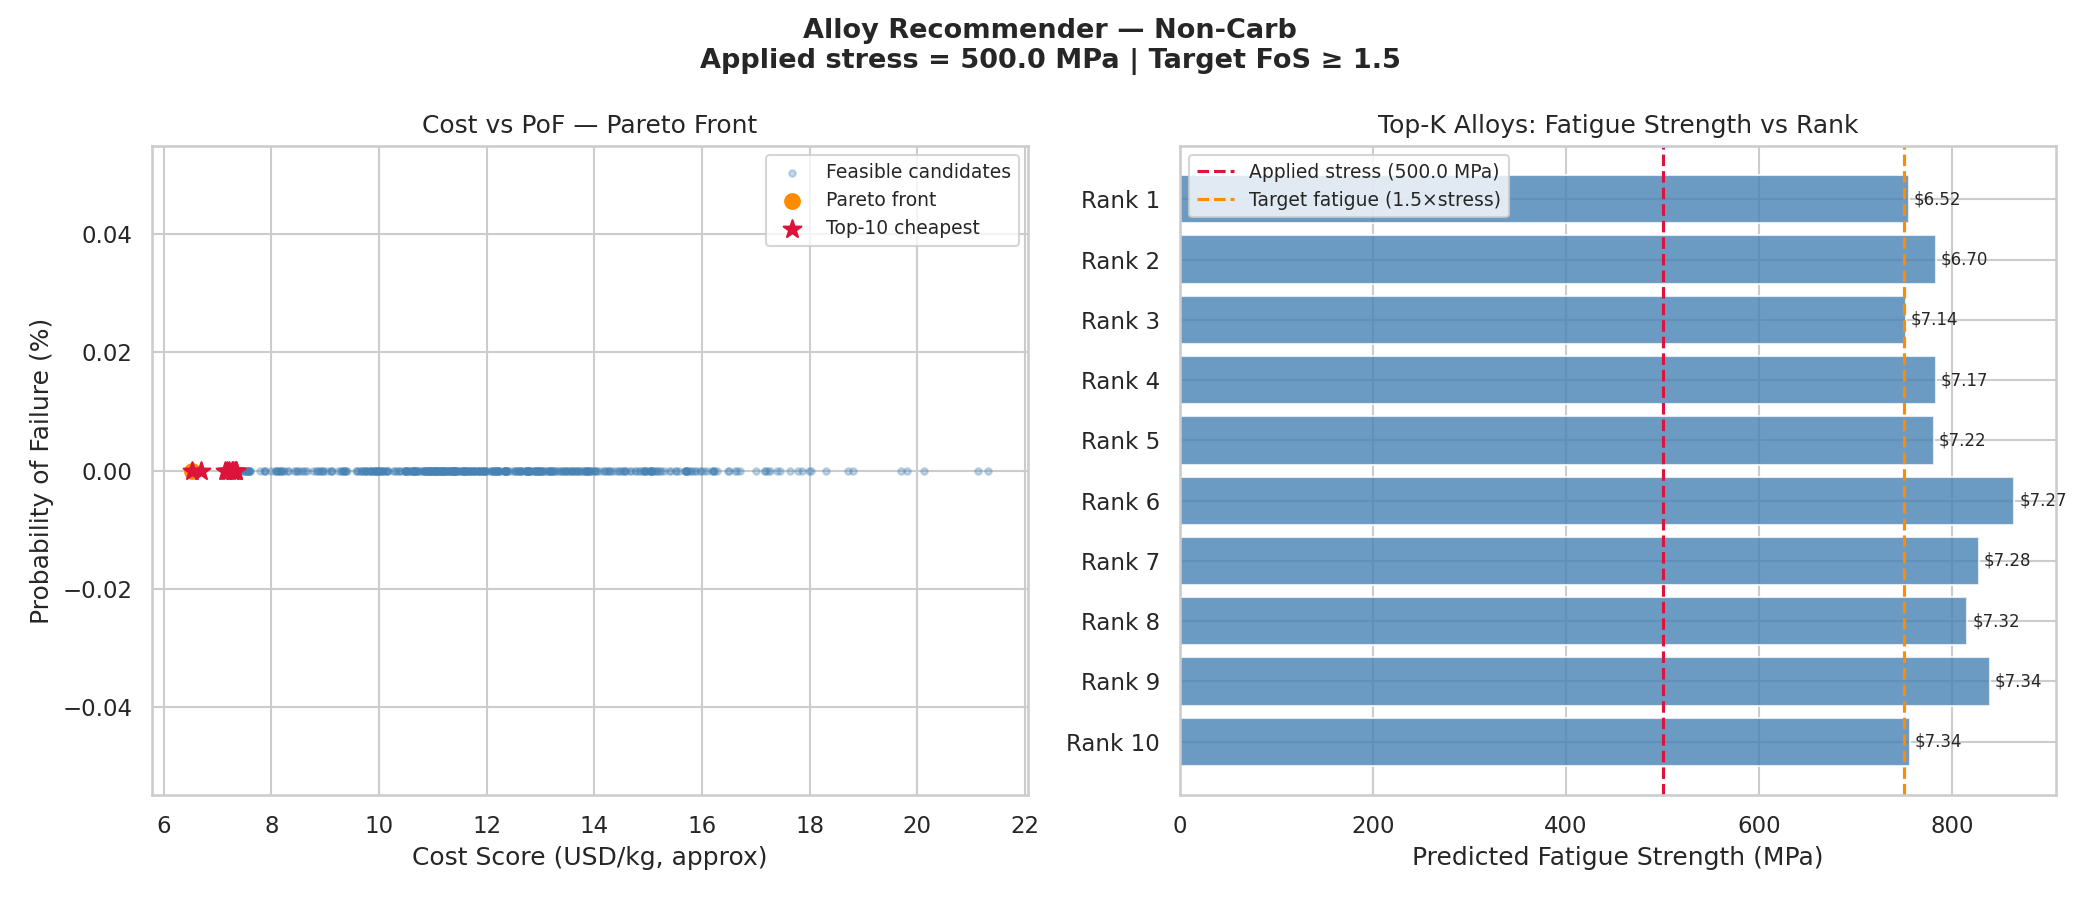
\includegraphics[width=\textwidth]{models/pareto_non_carb.png}
    \caption{Non-Carburised regime (500\,MPa, FoS\,$\geq 1.5$).}
  \end{subfigure}
  \hfill
  \begin{subfigure}[b]{0.49\textwidth}
    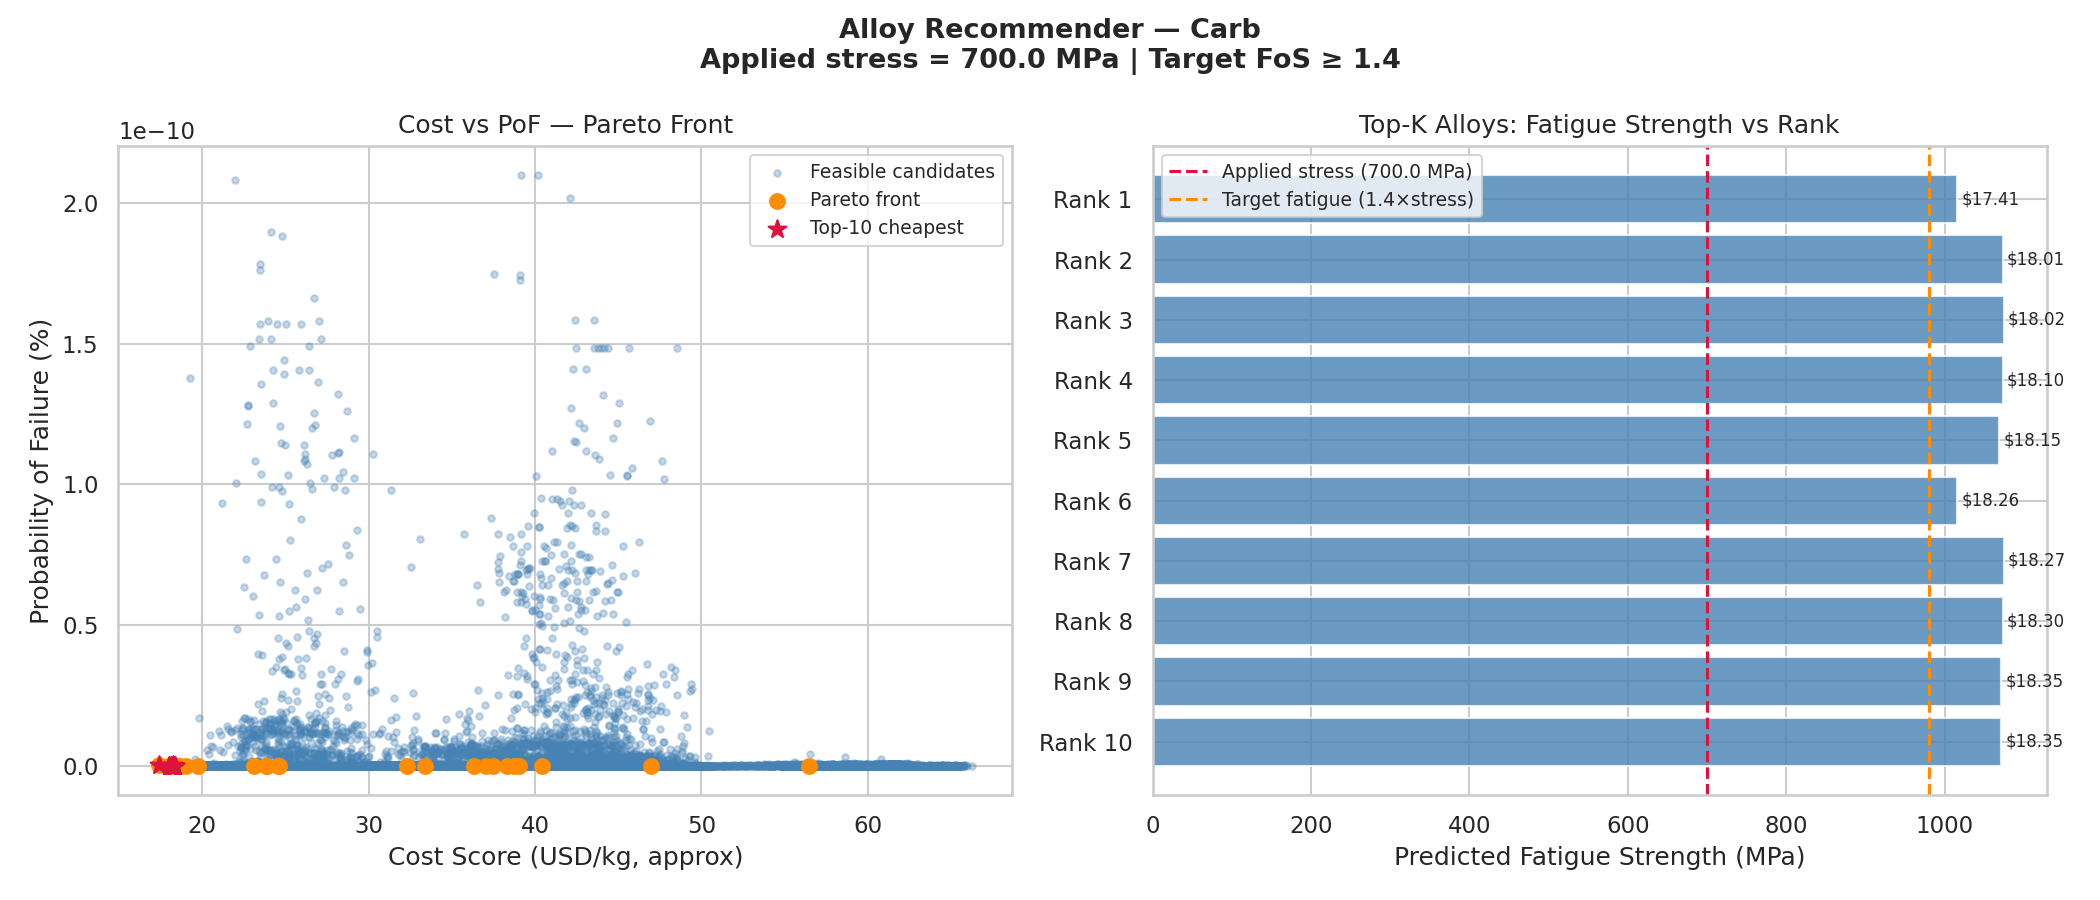
\includegraphics[width=\textwidth]{models/pareto_carb.png}
    \caption{Carburised regime (700\,MPa, FoS\,$\geq 1.4$).}
  \end{subfigure}
  \caption{Pareto front (cost vs.\ PoF). Orange dots: Pareto-optimal alloys. Red stars: top-$K$
           cheapest feasible alloys. Right sub-panel: predicted fatigue vs.\ rank.}
  \label{fig:pareto}
\end{figure}

\subsection{Pareto Front Analysis}

7 non-dominated alloys were identified for the non-carburised regime and 18 for the carburised
regime. The Pareto front reveals a clear \textit{cost--reliability tradeoff}: adding Mo
(+\$30/kg) shifts the PoF from $\sim$0.01\% to essentially zero while increasing cost by
$\sim$\$3/kg. For most structural applications (target PoF\,$< 1\%$), Mo can be eliminated
entirely, saving significant cost.


% ─────────────────────────────────────────────────────────────────────────────
\section{Deployment: Streamlit Application}
% ─────────────────────────────────────────────────────────────────────────────

A two-tab interactive GUI (\texttt{app.py}) was built using Streamlit and deployed locally.

\subsection{Tab 1 — Forward Prediction}

The engineer inputs all 26 feature values via sliders, specifies the applied operational stress,
and clicks ``Predict''. The app returns:
\begin{itemize}[nosep]
  \item Metric cards: predicted fatigue, FoS, PoF, active regime.
  \item Gaussian distribution plot with applied stress marker, failure-area shading, and 95\% PI.
  \item SHAP waterfall bar chart for the specific input showing top-10 feature contributions.
\end{itemize}

\subsection{Tab 2 — Inverse Design}

The engineer specifies regime, applied stress, target FoS, maximum PoF, and sample size. The app:
\begin{itemize}[nosep]
  \item Runs the neighbourhood sampler + kNN hull filter.
  \item Returns Pareto scatter (cost vs.\ PoF) and ranked fatigue bar chart.
  \item Displays a formatted top-$K$ alloy table.
  \item Shows SHAP waterfall for any selected rank (interactive dropdown).
  \item Outputs a cost breakdown table for Rank \#1.
\end{itemize}

All models are loaded from disk at startup via \texttt{joblib} and cached with
\texttt{@st.cache\_resource}, ensuring sub-second response after the first load.


% ─────────────────────────────────────────────────────────────────────────────
\section{Discussion}
% ─────────────────────────────────────────────────────────────────────────────

\subsection{What Worked}

\begin{enumerate}[nosep]
  \item \textbf{Regime split} was the single highest-impact decision. Global models (Linear,
        Ridge, Lasso) could not capture the bimodal distribution; splitting by carburising status
        reduced RMSE by $\sim$30\%.
  \item \textbf{Honest CV evaluation} exposed the carburised model's overfit in v1.0 (RMSE
        27.2\,MPa single-split vs.\ 40.4\,MPa cross-validated). This is a critical finding: a
        model that appears excellent on a single split may be unreliable in production.
  \item \textbf{Neighbourhood sampling} solved the curse of dimensionality in inverse design that
        made Latin Hypercube Sampling impractical ($<0.01\%$ survival rate).
  \item The \textbf{kNN hull guard} prevents the recommender from returning metallurgically
        impossible or untested alloy configurations.
\end{enumerate}

\subsection{Limitations and Future Work}

\begin{enumerate}[nosep]
  \item \textbf{Carburised data scarcity} ($N=48$) limits prediction reliability
        (CV std = 14.6\,MPa). Acquiring 50--100 additional carburised samples would likely halve
        the uncertainty.
  \item \textbf{Normality of NC residuals} fails on out-of-fold (OOF) predictions
        (Shapiro--Wilk $p < 0.001$, KS $p = 0.0002$), producing a Gaussian PoF that differs
        from the empirical PoF by up to 7 percentage points near the fatigue limit.
        The v2.0+ code uses an empirical CDF of OOF residuals for NC PoF; Gaussian is retained
        for the carburised regime (OOF residuals pass normality).
  \item \textbf{Applicability boundary}: the NIMS dataset consists predominantly of
        alloyed low-alloy steels (Cr, Mn, Mo, Ni present). External validation against
        handbook data shows that plain-carbon grades (e.g.\ AISI 1045 normalised) are
        over-predicted by $\sim$190\,MPa. The model should not be used for steels with
        Cr\,+\,Ni\,+\,Mo\,$<$\,0.1\,wt\%.
  \item \textbf{Cost model} uses fixed elemental prices. Integration with live LME API data
        would make the recommender directly useful for procurement decisions.
  \item \textbf{Physical constraints} on composition (e.g.\ hardenability rules, weldability
        limits) are not yet encoded. Adding metallurgical feasibility constraints as hard filters
        would improve recommendations.
  \item \textbf{Fatigue ratio model}: the dataset records rotating-bending fatigue. Extension
        to axial or torsional fatigue would require a separate target or a correction-factor model.
\end{enumerate}


% ─────────────────────────────────────────────────────────────────────────────
\section{Conclusion}
% ─────────────────────────────────────────────────────────────────────────────

We developed a complete, production-ready data-driven fatigue strength prediction system for
low-alloy steels. The key contributions are:

\begin{enumerate}[nosep]
  \item A \textbf{Mixture-of-Experts architecture} (XGBoost for non-carburised, Random Forest for
        carburised) with regime-specific VIF$\to$SHAP feature selection.
  \item \textbf{Honest performance evaluation} via nested cross-validation with Optuna tuning,
        achieving a 5-fold CV RMSE of \textbf{19.9\,MPa} for the non-carburised regime.
  \item A \textbf{reliability wrapper} mapping predictions to Probability of Failure, validated
        with residual normality tests.
  \item An \textbf{inverse design engine} combining neighbourhood sampling, kNN hull filtering,
        and Pareto-front analysis to recommend the cheapest viable alloy configuration for any
        operating condition.
  \item An interactive \textbf{Streamlit GUI} integrating all components for real-time use by
        materials engineers.
\end{enumerate}

The system demonstrates that data-driven models can replace expensive physical fatigue testing for
alloy screening, while the inverse design module enables cost-optimal alloy selection — a direct
contribution to sustainable manufacturing.

% ─────────────────────────────────────────────────────────────────────────────
\appendix
\section{File Structure}
% ─────────────────────────────────────────────────────────────────────────────

\begin{lstlisting}
Project/
  data.csv                  NIMS dataset (437 samples, 26 features)
  Project 1.0.py            Baseline MoE models (single-split)
  Project 2.0.py            Phase 1: nested CV + Optuna + residual diagnostics
  Project 3.0.py            Phase 2+3: inverse design + cost/Pareto analysis
  app.py                    Phase 4: Streamlit GUI
  models/
    nc_xgb.pkl              Tuned XGBoost — non-carburised
    c_rf.pkl                Tuned Random Forest — carburised
    nc_features.json        Selected feature list — non-carburised
    c_features.json         Selected feature list — carburised
    metadata.json           CV RMSE, std, best hyperparameters
    residual_diagnostics.png
    pareto_non_carb.png
    pareto_carb.png
\end{lstlisting}

% ─────────────────────────────────────────────────────────────────────────────
\begin{thebibliography}{9}
\bibitem{agrawal2014}
  A.~Agrawal, P.~D.~Deshpande, A.~Cecen, G.~P.~Basavarsu, A.~N.~Choudhary, S.~K.~Kalidindi,
  ``Exploration of data science techniques to predict fatigue strength of steel from composition
  and processing parameters,''
  \textit{Integrating Materials and Manufacturing Innovation}, vol.~3, no.~1, pp.~1--19, 2014.
\end{thebibliography}

\end{document}
